% Created 2024-12-11 Wed 10:10
% Intended LaTeX compiler: pdflatex
\documentclass[11pt]{article}
\usepackage[utf8]{inputenc}
\usepackage[T1]{fontenc}
\usepackage{graphicx}
\usepackage{longtable}
\usepackage{wrapfig}
\usepackage{rotating}
\usepackage[normalem]{ulem}
\usepackage{amsmath}
\usepackage{amssymb}
\usepackage{capt-of}
\usepackage{hyperref}
\usepackage{minted}
\usepackage[margin=0.5in]{geometry}
\hypersetup{colorlinks, linkcolor=black}
\usepackage{geometry}
\geometry{top=2cm}
\geometry{bottom=2cm}
\usepackage{fancyhdr}
\pagestyle{fancy}
\fancyhf[L]{Sistemas Operativos en Red}
\fancyhf[R]{Tema 01}
\fancyfoot[R]{ismael.macareno@educa.madrid.org}
\fancyfoot[L]{CC BY-NC-SA 4.0}
\usepackage{parskip}
\usepackage{mdframed}
\usepackage{fancyvrb}
\usepackage{xcolor}
\definecolor{shadecolor}{RGB}{220,220,220}
\newenvironment{shadedcode}{%
\VerbatimEnvironment
\begin{mdframed}[backgroundcolor=shadecolor,linewidth=0pt]}%
{\end{mdframed}}
\usepackage{attachfile2}
\newcommand{\textattachfilecolor}[2]{\textattachfile[color=0 0 0.5]{#1}{\textcolor{blue}{#2}}}
\usepackage[spanish]{babel}
\usepackage{datetime2}
\DTMlangsetup[es-ES]{ord=raise}
\renewcommand{\dateseparator}{/}
\usepackage{titlesec}
\usepackage{afterpage}
\newcommand\blankpage{\null\thispagestyle{empty}\newpage}
\usepackage{colortbl}
\usepackage{pdfpages}
\usepackage{tcolorbox}
\usepackage{listings}
\usepackage[spanish]{babel}
\lstset{
inputencoding=utf8,
extendedchars=true,
literate={ñ}{{\~n}}1 {Ñ}{{\~N}}1 {á}{{\'a}}1 {é}{{\'e}}1 {í}{{\'i}}1 {ó}{{\'o}}1 {ú}{{\'u}}1 {Á}{{\'A}}1 {É}{{\'E}}1 {Í}{{\'I}}1 {Ó}{{\'O}}1 {Ú}{{\'U}}1,
basicstyle=\ttfamily,
breaklines=true,
columns=fullflexible,
keepspaces=true,
language=TeX,
morekeywords={*, -, **, /}
}
\author{Ismael Macareno Chouikh}
\date{\today}
\title{Examen \emph{Bash Scripting} Completo - Nivel Básico}
\hypersetup{
 pdfauthor={Ismael Macareno Chouikh},
 pdftitle={Examen \emph{Bash Scripting} Completo - Nivel Básico},
 pdfkeywords={},
 pdfsubject={},
 pdfcreator={Emacs 29.4 (Org mode 9.6.15)}, 
 pdflang={Spanish}}
\begin{document}

\maketitle

\section{Menú \texttt{Bash} básico}
\label{sec:org605a561}
\begin{figure}[htbp]
\centering
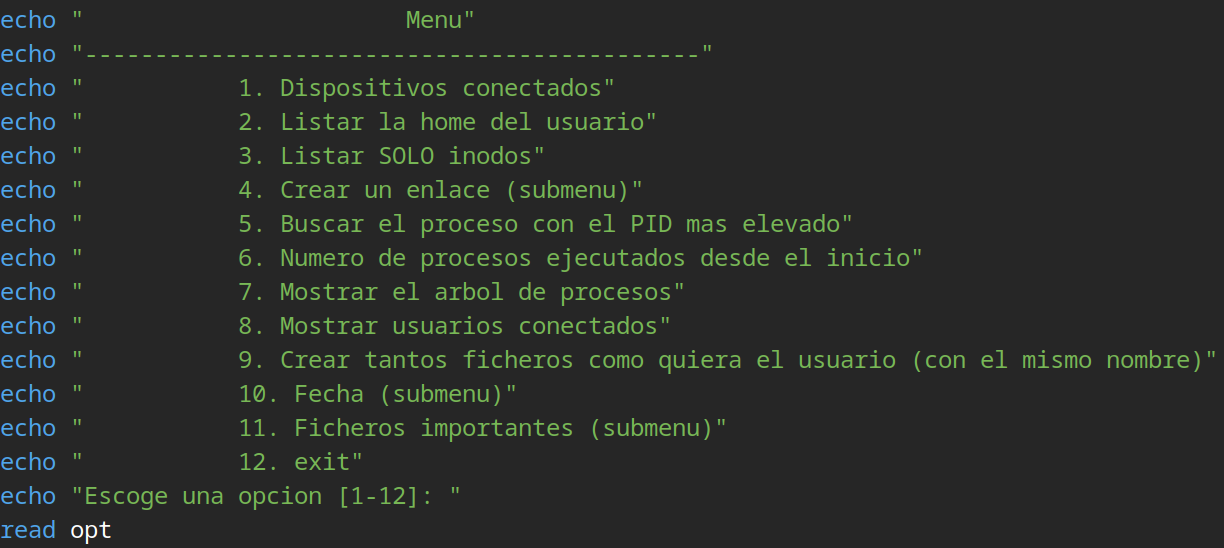
\includegraphics[width=.9\linewidth]{../examenes/img/ejemplo-script-menu-basico.png}
\caption{Macareno, Ismael. (2024). Ejemplo Menú \texttt{Bash} para examen [PNG]. Propia}
\end{figure}

Se solicita que el alumno realice un menú \texttt{bash} como el que se puede ver en la imagen de arriba.

Cada una de las opciones tendrá una funcionalidad descrita a continuación:
\begin{enumerate}
\item Mostrará \textbf{solo} el nombre de los dispositivos conectados (Ej. /dev/loop1)
\item Listar la \texttt{\$HOME} del usuario que ejecute el script
\item Obtener los \textbf{inodos} de todo lo contenido en la \texttt{\$HOME} del usuario que ejecute el script
\item Se creará un \textbf{submenu} en el cual se darán dos opciones:
\begin{itemize}
\item Crear un enlace simbólico (se solicitará al usuario la ruta completa del \texttt{TARGET} y el \texttt{DIRECTORY})
\item Crear un enlace duro (se solicitará al usuario la ruta completa del \texttt{TARGET} y el \texttt{DIRECTORY})
\end{itemize}
\item Obtener el PID del proceso ejecutándose más elevado
\item Obtener el número de procesos que se han ejecutado desde que se inició el sistema
\item Mostrar el árbol de procesos
\item Mostrar los usuarios conectados
\item Crear un bucle en el cuál se le solicite al usuario un número de ficheros a crear y luego
crear cada uno de estos ficheros con un contenido en su interior (Ej. Fic1.txt, Fic2.txt, etc)
\item Crear un \textbf{submenu} en el cuál se darán las siguientes opciones:
\begin{itemize}
\item Dar la fecha completa (Ej. Wed Dec 11 10:03:59 AM CET 2024)
\item Dar solo la Fecha (Ej.2024-12-11)
\item Dar solo la hora (Ej. 10:04:55)
\item Dar el día de la semana (Ej. 11)
\item Dar el mes del año (Ej. 12)
\item Dar el año (Ej. 2024)
\end{itemize}
\item Crear un submenu con las siguientes opciones
\begin{itemize}
\item Sacar \textbf{solo el nombre} de todos los usuarios del sistema
\item Sacar \textbf{solo} los \emph{\texttt{hashes}} de las contraseñas de los usuarios del sistema
\end{itemize}
\item Sacar por pantalla al usuario el mensaje \textbf{Gracias por ejecutarme} y cerrar el programa
\end{enumerate}


El programa deberá ejecutarse todo el rato hasta que el usuario quiera salir usando la opción
número 12.
\end{document}
